
\documentclass[12pt]{article}
\usepackage{amsmath}
\DeclareMathOperator*{\argmin}{arg\,min} % thin space, limits underneath in displays
\DeclareMathOperator*{\argmax}{arg\,max} % thin space, limits underneath in displays
\newtheorem{thm}{Theorem}
\usepackage{amssymb}
\usepackage{amsfonts}
\usepackage{mathrsfs}
\usepackage{bm}
\usepackage{indentfirst}
\setlength{\parindent}{0em}
\usepackage[margin=1in]{geometry}
\usepackage{graphicx}
\usepackage{setspace}
\doublespacing
\usepackage[flushleft]{threeparttable}
\usepackage{booktabs,caption}
\usepackage{float}
\usepackage{graphicx}
\usepackage[sort,comma]{natbib}

\usepackage{import}
\usepackage{xifthen}
\usepackage{pdfpages}
\usepackage{transparent}

\newcommand{\incfig}[1]{%
\def\svgwidth{\columnwidth}
\import{./figures/}{#1.pdf_tex}
}




\title{Econ8410 Course paper}
\author{Yan Hao}
\date{Dec. 5, 2021}


\begin{document}
\maketitle




\section{Introduction}
I will reproduce most part of the Sheffrin and Woo's results in this course paper. It
includes six countries, United Kingdom, Thailand, Sweden, United States, Canada, and
Denmark (KTSUCD). Balance of Payment data are from International Monetary Fund. Data 
using to compute Net output are from Penn World Table and cover the period 1977-2019 
(42 years).


\section{Theoretical Model}
Similar to what we discussed in class the model assumes that 1) there is a small open 
economy with a given world interest rate; 2) Consumption depends solely on a country's
wealth; 3) The wealth is measured by the sum of NO and the stock of external assets (B);
4) The first order difference of NO is stationary, which implies the level of current
account is stationary; 5) Agents cannot borrow money without a limit (Transversality 
condition)
\begin{equation*}
\lim_{i \to \infty} \left( \frac{1}{1 + r} \right) ^{i}	b_{t + i} = 0, 
\end{equation*}
where $ \beta = \frac{1}{1 + r} $, and $ b_{t + i} $ is the stock of external assets
at the begining of period $ t + i $.


The accumulation of external assets follows the rule below:
\begin{equation}
b_{t + i} = (1 + r)b_{t} + \left[ y_{t} - c_{t} - i_{t} - g_{t} \right].
\end{equation}

By iterating equation (1),

\begin{align*}
b_{t} &= \frac{1}{1 + r}b_{t + 1} - \frac{1}{1 + r}(y_{t} - c_{t} - i_{t} - g_{t})\\
 &= \beta b_{t + 1} -  \beta x_{t}, \text{ where $ x_{t} = y_{t} - c_{t} - i_{t} - 
 g_{t}$ is the net export }\\
 &= \beta(\beta b_{t + 2} - \beta x_{t + 1}) - \beta x_{t}\\
 &= \beta^{2} b_{t + 2} - \beta^{2} x_{t + 1}  - \beta x_{t}\\
 &...\\
\end{align*}
\begin{equation}
b_{t} =  - \sum\limits_{i = 1} ^\infty \beta^{i} x_{t + i - 1}	.
\end{equation}

It says the external asset in period $ t $ is the present discounted value of the 
stream of future trade deficits.


The consumption for individual agent is the difference between income and the sum
of investment, government spending, and net export,

\begin{equation}
c_{t + i - 1} = y_{t + i - 1} - i_{t + i - 1} - g_{t + i - 1} - x_{t + i - 1}.
\end{equation}
The sum of present discounted value can be written as

\begin{equation}
\sum\limits_{i = 1} ^\infty \beta^{i} c_{t + i - 1} = \sum\limits_{i = 1} ^\infty 
\beta^{i} [y_{t + i - 1} - i_{t + i - 1} - g_{t + i - 1}] - 
\sum\limits_{i = 1} ^\infty \beta^{i}x_{t + i - 1}.
\end{equation}

Plug in equation (2), we obtain agent's intertemporal budget constraint,
\begin{equation}
\sum\limits_{i = 1} ^\infty \beta^{i} c_{t + i - 1} =\left( 
\sum\limits_{i = 1} ^\infty 
\beta^{i} (NO)_{t + i - 1}\right) 
 + b_{t},
\end{equation}
where the Net Output ($ NO $) is defined as GDP less the sum of investment plus 
government spending, $ NO = Y - (I + G) $.

Now we can write down the optimization problem:

\begin{align*}
&U = {\rm I\!{E}}_{0}\left( \sum\limits_{i = 0} ^\infty \beta^{i} u(c_{i})	 \right)\\
& s.t. \quad
\sum\limits_{i = 1} ^\infty \beta^{i} c_{t + i - 1} =\left( 
\sum\limits_{i = 1} ^\infty 
\beta^{i} (NO)_{t + i - 1}\right) 
 + b_{t}.
\end{align*}


With quadratic utility funtion, we can find the closed-form solution for consumption,
\begin{equation}
c_{t} = \frac{r}{1 + r}\left\{ 
(1 + r)b_{t} + \sum\limits_{i = 0} ^\infty \left( \frac{1}{1 + r} \right)^{i}
{\rm I\!{E}}_{t}(NO_{t + i})
\right\}.
\end{equation}



Current account is the difference between savings and investment, and it can be
written as a function of net output,

\begin{equation}
CA_{t} = S_{t} - I_{t} = y_{t} + r b_{t}  - i_{t} - g_{t} - c_{t} = NO_{t} + r b_{t} - 
c_{t}.
\end{equation}


Plug in equation (6), we can rewrite $ CA $ as a function of the change of $ NO $,
\begin{align}
CA_{t} &= NO_{t} + r b_{t} - \left\{ 
\frac{r}{1 + r}\left\{ 
(1 + r)b_{t} + \sum\limits_{i = 0} ^\infty \left( \frac{1}{1 + r} \right)^{i}
{\rm I\!{E}}_{t}(NO_{t + i})
\right\} 
\right\} \\
 &=  - \left( \frac{r}{1 + r} \right) \sum\limits_{i = 0} ^\infty 
 \left( \frac{1}{1 + r} \right) ^{i}{\rm I\!{E}}_{t}(NO_{t + i} - NO_{t})\\
 &=  - \sum\limits_{i = 1} ^\infty \left( \frac{1}{1 + r} \right)^{i}{\rm I\!{E}}_{t}
 (\Delta NO_{t + i}) .
\end{align}

Clearly, $ \Delta NO $ is the first difference of $ NO $. If it is stationary, then
the current account will also be stationary in its level. We will examine this latter.


\section{Regression Model}

To test this theoretical result (equation (10)), we can run a second-order vector 
autoregression (VAR) to capture the properties of the series. The VAR can be written
as the following,

\begin{equation}
\begin{bmatrix}
\Delta NO_{t}\\
\Delta NO_{t - 1}\\
CA_{t}\\
CA_{t - 1}
\end{bmatrix}
=
\begin{bmatrix}
a_1 & a_2 & b_1 & b_2\\
1 & 0 & 0 & 0\\
c_1 & c_2 & d_1 & d_2\\
0 & 0 & 1 & 0
\end{bmatrix}
\begin{bmatrix}
\Delta NO_{t - 1}\\
\Delta NO_{t - 2}\\
CA_{t - 1}\\
CA_{t - 2}
\end{bmatrix}
 + 
\begin{bmatrix}
u_{t}\\
0\\
v_{t}\\
0
\end{bmatrix},
\end{equation}
or it can be written in a compact form, $ Z_{t} = AZ_{t - 1} + w_{t} $, where
$ {\rm I\!{E}}(Z_{t + i}) = A^{i}Z_{t} $ (This can be derived by iterating the equation
of $ Z_{t} $, then take the expectation of it). Considering the restrictions on 
current account, equation (10), we can write the following,

\begin{align*}
CA_{t} &=  - \sum\limits_{i = 1} ^\infty \left( \frac{1}{1 + r} \right) ^{i}
{\rm I\!{E}}_{t}(\Delta NO_{t + i})\\
\bm{CA}_{t}' &=  - \sum\limits_{i} \left( \frac{1}{1 + r} \right)^{i} \bm{h}'\bm{A}^{i}
\bm{Z}_{t}\\
 &= - \bm{h}' \sum\limits_{i} \left( \frac{\bm{A}}{1 + r} \right)^{i} \bm{Z}_{t}\\
 &= \bm{K} \bm{Z}_{t},
\end{align*}
where $ \bm{h}' = [1,0,0,0] $,
\begin{equation*}
\bm{K} =  - \bm{h}' \frac{\left( \frac{\bm{A}}{1 + r} \right) }{
		\left[ 1 - \left( \frac{\bm{A}}{1 + r} \right)  \right] 
}.
\end{equation*}



We know $ \bm{h}' $ is a $ 1  \times 4 $ row vector, the ratio of $ \bm{A} $ is still
a $ 4  \times 4 $ matrix. Therefore, $ \bm{K} $ is a $ 1  \times 4 $ row matrix, 
$ \bm{Z_{t}} $ is a $ 4  \times  1 $ matrix,
\begin{align*}
		\bm{K} &= \begin{bmatrix}
				\gamma_1 &\gamma_2 &\gamma_3 &\gamma_4
		\end{bmatrix}\\
		\bm{Z_{t}} &= \begin{bmatrix}
				\Delta NO_{t}\\
				\Delta NO_{t - 1}\\
				CA_{t}\\
				CA_{t - 1}
		\end{bmatrix}
\end{align*}

Hence, we would like to see $ \gamma_1, \gamma_2, \text{ and } \gamma_4 $ are zeros.
And we can use this to predict the current account series, then evaluate the performance
of the model by comparing the prediction of $ CA $ series and the actual ones.



\section{Estimations, and results}
As we discussed in section 2, we want to first check if the first difference of $ NO $
and the level of $ CA $ are stationary. This can be done by running regressions
of the form:

\begin{equation}
\Delta \bm{NO}_{t} = a + b_1 \Delta \bm{NO}_{t - 1} + b_2 \Delta \bm{NO}_{t - 2} + c
\bm{NO}_{t - 1} + d \cdot time  + \eta_{t},
\end{equation}

and test if the coefficient $ c $ is negative and significantly different than zero
using the Dickey-Fuller statistics, $ \tau_{\tau} $. For the net output series,
we want to fail to reject the null; for the current account series, we would like to
reject the null. Since we have 42 observations, criterion for sample size of 50 could
be the appropriate one. The critical values for 10\% and 5\% significant level are
-3.18 and -3.5.

For KTSUCD countries, $ t $ statistics for the net output series are -1.833, -1.532,
-0.868, -2.986, -0.997, -1.914. Except for the United States, these are below the 
critical value to reject the null. For the current account series, statistics for 
KTSUCD countries are -3.805, -2.924, -2.361, -2.215, -1.951, -1.573.

Table 1 to Table 6 present the result of VAR and the estimated K matrix for KTSUCD 
countries. Figure 1 to Figure 6 are the comparison between the prediction based on
vector $ \bm{K} $ and the actual current account series (Dashed-line: prediction, 
Solid line: actual series). Except for Sweden and Denmark,
other four countries are run in a current account deficits during this period. Denmark's
current account series is exploding. 
From the figure, even though the $ \bm{K} $ vector for the US does not satisfy the
requirements of theoretical model, the prediction of it performs well.


\begin{table}[h!]
\begin{center}
\caption{United Kingdom}			
\begin{threeparttable}

\begin{tabular}{lcccc}
&$ \Delta NO_{t} $        &$ CA_{t} $				 &4\%				&14\% \\
\hline \\[-1.8ex]

$ \Delta NO_{t - 1} $   & 0.215    &-0.010     &-0.682	&	-0.695  \\
				                &(0.162)   &(0.071)    &        &         \\
$ \Delta NO_{t - 2} $   & 0.267    &-0.102     & 0.367  &  0.353  \\
				                &(0.159)   &(0.070)    &        &         \\
$ CA_{t - 1} $          &-0.069    & 1.072     &-3.819  & -3.672  \\
				                &(0.381)   &(0.167)    &        &         \\
$ CA_{t - 2} $          & 0.002    &-0.124     & 4.590  &  4.413  \\
				                &(0.393)   &(0.173)    &        &         \\
$ R^{2} $				        & 0.188    & 0.925     &        &         \\
\hline \\[-1.8ex]


\end{tabular}


\end{threeparttable}
\end{center}
\end{table}







\begin{table}[h!]
\begin{center}
\caption{Thailand}			
\begin{threeparttable}

\begin{tabular}{lcccc}
&$ \Delta NO_{t} $        &$ CA_{t} $				 &4\%				&14\% \\
\hline \\[-1.8ex]

$ \Delta NO_{t - 1} $   & 0.779    &-0.078     &-0.077	&-0.041	  \\
				                &(0.167)   &(0.063)    &        &         \\
$ \Delta NO_{t - 2} $   &-0.069    &-0.130     &-0.935  &-0.971   \\
				                &(0.191)   &(0.072)    &        &         \\
$ CA_{t - 1} $          & 0.311    & 0.553     & 2.946  & 3.061   \\
				                &(0.425)   &(0.160)    &        &         \\
$ CA_{t - 2} $          &-0.660    & 0.055     &-2.362  &-2.455   \\
				                &(0.390)   &(0.147)    &        &         \\
$ R^{2} $				        & 0.676    & 0.831     &        &         \\
\hline \\[-1.8ex]


\end{tabular}


\end{threeparttable}
\end{center}
\end{table}






\begin{table}[h!]
\begin{center}
\caption{Sweden}			
\begin{threeparttable}

\begin{tabular}{lcccc}
&$ \Delta NO_{t} $        &$ CA_{t} $				 &4\%				&14\% \\
\hline \\[-1.8ex]

$ \Delta NO_{t - 1} $   & 0.507    &-0.059     & 1.616 	 & 1.551	  \\
				                &(0.174)   &(0.119)    &         &         \\
$ \Delta NO_{t - 2} $   & 0.276    & 0.113     &-1.238   &-1.207   \\
				                &(0.176)   &(0.120)    &         &         \\
$ CA_{t - 1} $          & 0.097    & 0.963     &-3.685   &-3.592   \\
				                &(0.265)   &(0.181)    &         &         \\
$ CA_{t - 2} $          &-0.093    &-0.149     & 3.601   & 3.510   \\
				                &(0.279)   &(0.191)    &         &         \\
$ R^{2} $				        & 0.541    & 0.669     &         &         \\
\hline \\[-1.8ex]


\end{tabular}


\end{threeparttable}
\end{center}
\end{table}









\begin{table}[h!]
\begin{center}
\caption{United States}			
\begin{threeparttable}

\begin{tabular}{lcccc}
&$ \Delta NO_{t} $        &$ CA_{t} $				 &4\%				&14\% \\
\hline \\[-1.8ex]

$ \Delta NO_{t - 1} $   & 0.466     &-0.124     &-0.224 	&-0.240	  \\
				                &(0.158)    &(0.112)    &         &         \\
$ \Delta NO_{t - 2} $   & 0.284     & 0.110     &-0.094   &-0.092   \\
				                &(0.156)    &(0.110)    &         &         \\
$ CA_{t - 1} $          &-0.453     & 1.206     & 0.199   & 0.195   \\
				                &(0.229)    &(0.162)    &         &         \\
$ CA_{t - 2} $          & 0.370     &-0.224     & 0.352   & 0.345   \\
				                &(0.230)    &(0.163)    &         &         \\
$ R^{2} $				        & 0.731	    & 0.964     &         &         \\
\hline \\[-1.8ex]


\end{tabular}


\end{threeparttable}
\end{center}
\end{table}




\begin{table}[h!]
\begin{center}
\caption{Canada}			
\begin{threeparttable}

\begin{tabular}{lcccc}
&$ \Delta NO_{t} $        &$ CA_{t} $				 &4\%				&14\% \\
\hline \\[-1.8ex]

$ \Delta NO_{t - 1} $   &-0.086     &-0.063     &-0.194 	&-0.188	  \\
				                &(0.227)    &(0.080)    &         &         \\
$ \Delta NO_{t - 2} $   &-0.140     &-0.076     & 0.012   & 0.012   \\
				                &(0.159)    &(0.056)    &         &         \\
$ CA_{t - 1} $          &-0.341     & 1.222     & 0.403   & 0.406   \\
				                &(0.621)    &(0.220)    &         &         \\
$ CA_{t - 2} $          & 0.055     &-0.313     &-0.300   &-0.302   \\
				                &(0.656)    &(0.232)    &         &         \\
$ R^{2} $				        & 0.1       & 0.863     &         &         \\
\hline \\[-1.8ex]


\end{tabular}


\end{threeparttable}
\end{center}
\end{table}


\begin{table}[h!]
\begin{center}
\caption{Canada}			
\begin{threeparttable}

\begin{tabular}{lcccc}
&$ \Delta NO_{t} $        &$ CA_{t} $				 &4\%				&14\% \\
\hline \\[-1.8ex]

$ \Delta NO_{t - 1} $   & 0.505     & 0.134     &-0.461 	&	-0.458	  \\
				                &(0.202)    &(0.163)    &         &           \\
$ \Delta NO_{t - 2} $   &-0.020     &-0.061     & 0.048   &  0.048    \\
				                &(0.189)    &(0.152)    &         &           \\
$ CA_{t - 1} $          &-0.340     & 0.786     & 1.089   &  1.096    \\
				                &(0.226)    &(0.181)    &         &           \\
$ CA_{t - 2} $          & 0.403     & 0.270     &-0.750   & -0.755    \\
				                &(0.238)    &(0.191)    &         &           \\
$ R^{2} $				        & 0.198     & 0.946     &         &           \\
\hline \\[-1.8ex]


\end{tabular}


\end{threeparttable}
\end{center}
\end{table}





\begin{figure}[H]
\center{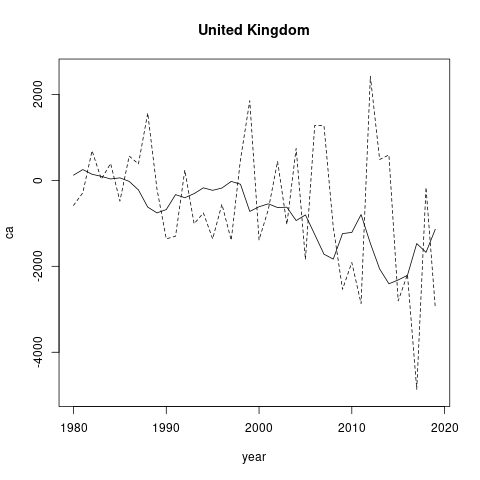
\includegraphics[scale =.5 ]  {figures/United_Kingdom.png}}
\caption{}
\end{figure}


\begin{figure}[H]
\center{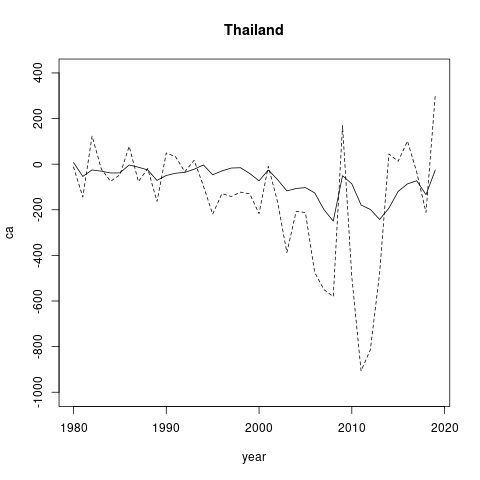
\includegraphics[scale =.5 ]  {figures/Thailand.png}}
\caption{}
\end{figure}


\begin{figure}[H]
\center{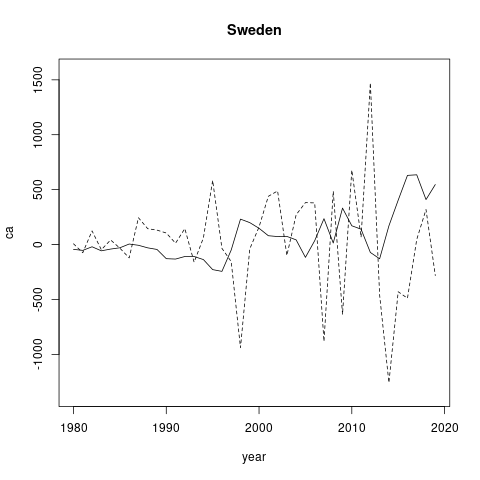
\includegraphics[scale =.5 ]  {figures/Sweden.png}}
\caption{}
\end{figure}


\begin{figure}[H]
\center{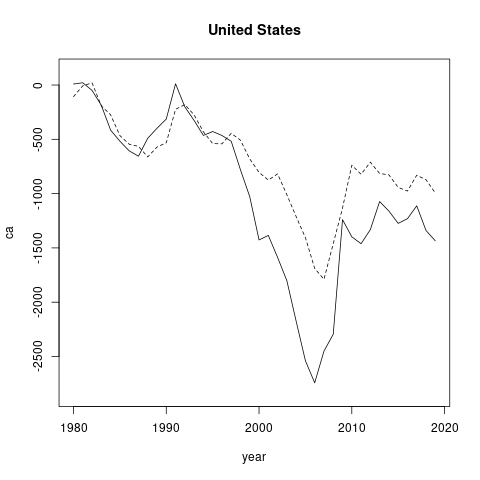
\includegraphics[scale =.5 ]  {figures/US.png}}
\caption{}
\end{figure}


\begin{figure}[H]
\center{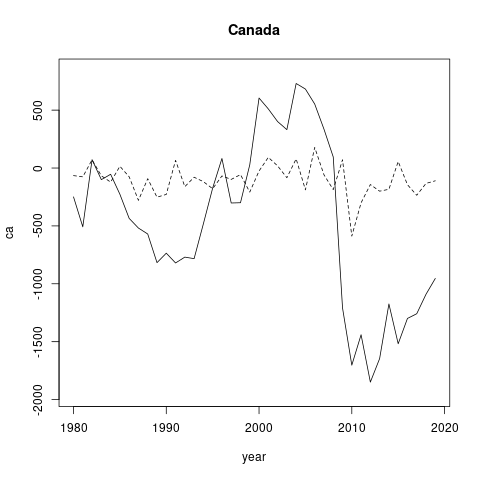
\includegraphics[scale =.5 ]  {figures/canada.png}}
\caption{}
\end{figure}


\begin{figure}[H]
\center{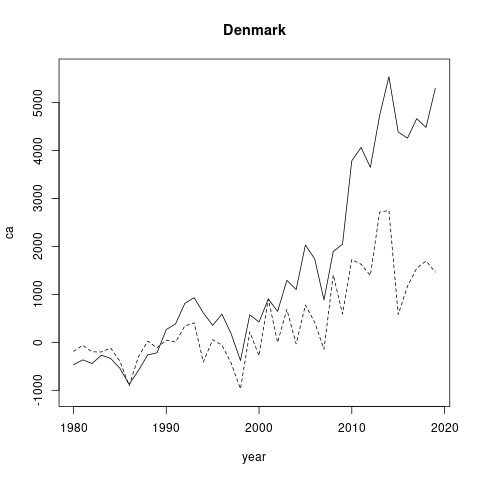
\includegraphics[scale =.5 ]  {figures/Denmark.png}}
\caption{}
\end{figure}






%\bibliographystyle{plainnat}
%\bibliography{my_bib}

\end{document}

